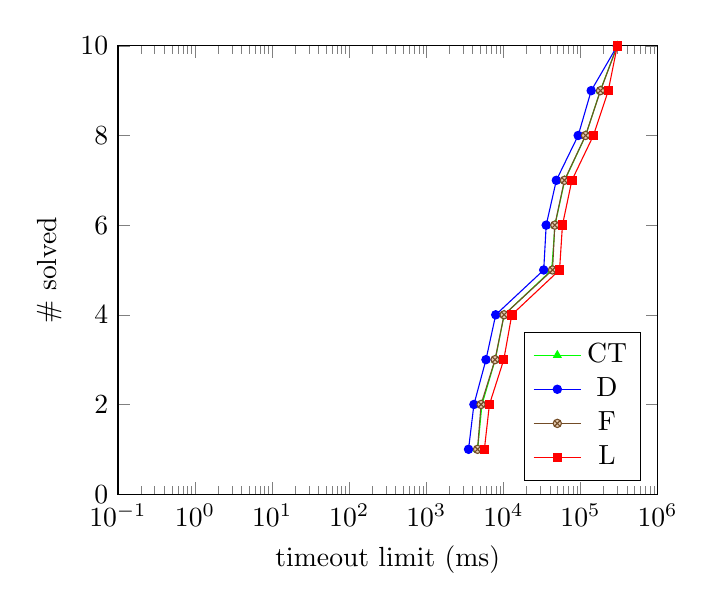
\begin{tikzpicture}[scale=1.0]
  \begin{axis}[
    xmode=log,
    ymin=0,ymax=10,
    xmin=0.1, xmax=1000000,
    every axis plot/.style={thin},
    xlabel={timeout limit (ms)},
    ylabel={\# solved},
    legend pos=south east
    % table/create on use/cumulative distribution/.style={
    %   create col/expr={\pgfmathaccuma + \thisrow{f(x)}}   
    % }
    ]
    \addplot 
    [mark=triangle*,
    mark size=1.5,
    mark options={solid},
    green] 
    coordinates {(4628.944, 1)
(5269.761, 2)
(7834.109, 3)
(10221.080, 4)
(42344.662, 5)
(46622.351, 6)
(62439.762, 7)
(116797.805, 8)
(180486.235, 9)
(300000.216, 10)};

    \addplot 
    [blue,
    mark=*,
    mark size=1.5,
    mark options={solid}]
    coordinates {(3528.185, 1)
(4146.147, 2)
(5942.940, 3)
(7947.450, 4)
(33338.965, 5)
(35886.866, 6)
(48586.026, 7)
(93315.398, 8)
(137662.304, 9)
(300000.350, 10)};

    \addplot [brown!60!black,
    mark options={fill=brown!40},
    mark=otimes*,
    mark size=1.5]
    coordinates {(4618.235, 1)
(5129.404, 2)
(7790.409, 3)
(10206.794, 4)
(43367.029, 5)
(46391.923, 6)
(61868.162, 7)
(116295.050, 8)
(181630.843, 9)
(300000.256, 10)};

    \addplot 
    [red,
    mark size=1.5,
    mark=square*]
    coordinates {(5663.567, 1)
(6586.833, 2)
(10111.497, 3)
(12848.274, 4)
(53494.054, 5)
(58301.293, 6)
(77295.794, 7)
(147053.910, 8)
(229203.930, 9)
(300000.278, 10)};
    \legend{CT,D,F,L}
  \end{axis}
\end{tikzpicture}
